        \subsection{Replikace}
        \label{kReplikace}
Replikace je proces, u kterého jsou data a databázové objekty kopírované z jednoho databázového serveru na druhý a poté synchronizovány pro zachování souladu obou databází. Synchronizací v tomto případě myslíme kopírováním všech změn, které v databázi nastanou. Použitím databáze je možno data distribuovat na různě vzdálená místa nebo mezi mobilní uživatele v rámci počítačové sítě a internetu \citep{Microsoft2013}.

Mnohé moderní aplikace se musí zabývat velkým počtem přístupů do databáze, což může v některých případech způsobovat problémy. Buď je server přetížen počtem připojení a data tedy přicházejí k uživateli pomalu, nebo dokonce úplně vypadne. 

Mezi časté důvody použití databázové replikace tedy patří zajištění dostupnosti dat\footnote{angl. High Availability}, resp. snížení pravděpodobnosti, že data nebudou dostupná, což může být způsobeno již zmíněným výpadkem serveru nebo například fyzickou ztrátou dat \citep{ObeHsu2012}. Další důvodem je rozložení zátěže přístupů do databáze mezi více serverů, takže nebude docházet ke zpomalení výkonu hlavního serveru ani k situaci, že data nebudou dostupná kvůli jeho výpadku \citep{BellKindahlThalmann2010}. Databáze je často zálohovaná, například skriptem dump a i to může server zpomalit. Vhodným řešením je tedy nejdříve vytvořit kopii dat na jiný datový server a až poté proces zálohování spustit. 

Všechny databáze zapojené do procesu replikace jsou v odborné literatuře nazývané uzly, v angličtině node. Tyto uzly dohromady tvoří replikační cluster\footnote{Volně přeloženo skupina serveru zapojených do replikace}. Při správně nastavené replikaci, by v clusteru nikdy neměly být méně než 3 uzly. Může se totiž stát, že vypadne jeden ze dvou uzlů, čímž dojde, ikdyž jen na krátkou chvíli, k situaci, že data nebudou v daný okamžik zálohovaná. 

Uzly v replikačním clusteru mohou mít jednu ze dvou základních rolí, nejčastěji nazývaných Master a Slave. Master server nebo pouze Master je server, který poskytuje data k replikaci, má práva na čtení i zápis a probíhají tedy na něm veškeré aktualizace. Je možno se setkat také s pojmenováním Primary server, Provider, Sender, Parent nebo Source server. Naprosto jiný pojem zavádí MS SQL Server, který tento zdrojový server nazývá Publisher (česky Vydavatel). Druhý databázový server je nejčastěji nazýván Slave, Standby, Reciever, Child nebo Subsciber (česky Odběratel). Poslední pojem je také používán MS SQL Serverem. Na tento server, který je dostupný vždy jen pro čtení dat, se data a aktualizace kopírují, není však možné na něj změny zapisovat \citep{RiggsKrossing2010}.

        %parametr H říká že to bude přímo na tom místě kde je v textu...více http://en.wikibooks.org/wiki/LaTeX/Floats,_Figures_and_Captions
          \begin{figure}[H]
            \centering
            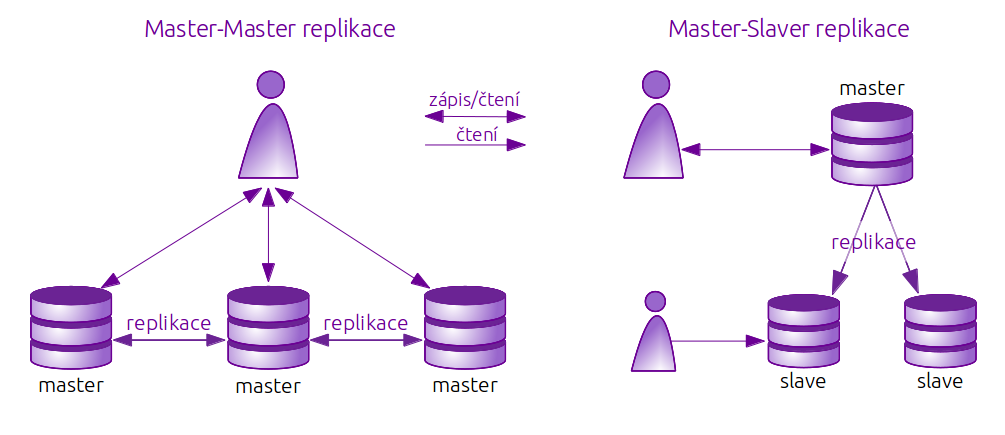
\includegraphics[scale=1]{../../../grafy/obr/schema_masterMasterSlave_maxiTence.png}
            \caption {Srovnání Master-Master a Master-Slave replikace}
            \label{srovnaniM-M-S}
          \end{figure}

Podle počtu Master a Slave serverů v replikačním clusteru, se rozlišuje zda se jedná o jednosměrnou nebo obousměrnou replikaci. Tzv. Master-Master replikace umožňuje zapisovat do všech uzlů v replikačním clusteru, což může být praktické například při použití databáze offline \odkazObrazek{srovnaniM-M-S}. Změny se tedy synchronizují mezi všemi databázovými uzly. Tento způsob však nese značné komplikace, je potřeba řešit konflikty změn ve stejných datech a je relativně náročný na údržbu. Tato práce se zabývá použitím druhé způsobu, tzv Master-Slave replikace. Tato replikace používá vždy jen jeden Master server v clusteru a dva a více Slave servery. Kopie dat tedy probíhá jednosměrně, vždy z Master na Slave servery. Podle Bella (2010) mají moderní aplikace často více čtenářů než zapisovatelů, proto je zbytečné, aby se všichni čtenáři připojovali na stejnou databázi jako zapisovatelé a zpomalovali tím jejich práci \citep{BellKindahlThalmann2010}. Z toho důvodu je tedy použití Master-Slave replikace více než vhodné.

Při návrhu replikace je potřeba zamyslet se také nad tím, zda bude synchronní či asynchronní. Synchronní replikace neumožní, aby na Master serveru proběhla nová transakce, dokud se poslední transakce úspěšně neprovede na Slave serveru \citep{Boszormenyi2013}. Tento přístup zajistí, že žádná data nebudou v průběhu transakce ztracena. V některých případech tento způsob může zbytečně zpomalit rychlost přístupu do databáze, protože je nutno čekat na každou nedokončenou transakci. Zároveň může způsobit snížení dostupnosti databáze, protože v případě, že se například přeruší spojení mezi servery, nemůže na masteru proběhnout žádný další dotaz. Ale jistě si najde své opodstatění například při bankovních transakcí, kde je potřeba, aby všechny operace proběhly na obou stranách. V tomto případě je užití tohoto způsobu zcela nezbytné. 

Druhým způsobem je asynchronní replikace, při které se nová data mohou zapisovat na Master server, přestože ještě nedošlo k replikaci stávajících dat na Slave server \citep{ObeHsu2012}. To je sice za běžného provozu rychlejší, v některý případech však může způsobit nekonzistenci dat, například když proběhne transakce na Master serveru, který však spadne dřív, než se změna zapíše na Slave. V takovém případě se Slave změní na Master server, ale zároveň se nikdy nedozví o transakci, o které má uživatel informace, že proběhla v pořádku. 

        \begin{figure}[H]
          \centering
          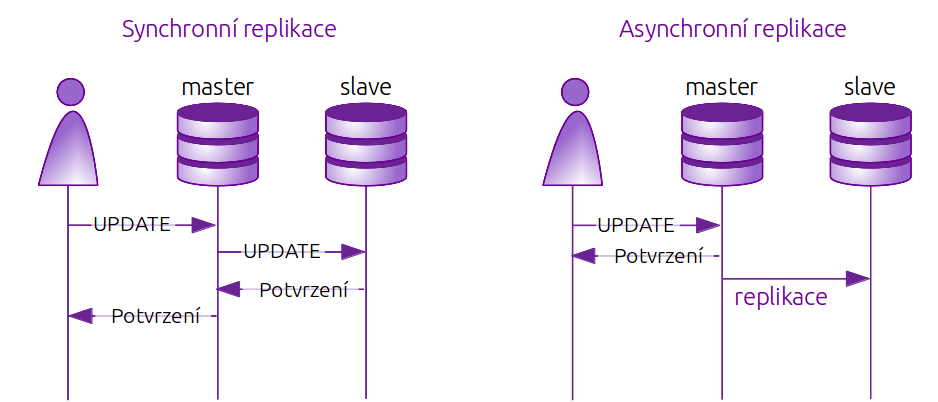
\includegraphics[scale=1]{../../../grafy/obr/schema_asyncSync_maxiTence.png}
          \caption {Rozdíl mezi synchronní a asynchronní replikací}
        \end{figure}

Replikace v PostgreSQL umožňuje plnou kopii dat z databáze i pouze výběr některých tabulek. Více o možnostech a způsobech nastavení replikace v kapitole \odkazKapitola{} a PRAKTICKÁ ČÁST :)
Dále je možno rozlišovat replikaci pole toho, zda je logická nebo fyzická. Výsledek obou typů má naprosto identický výsledek, přesto se mírně liší. 

Fyzická replikace kopíruje data na druhý server v binární podobě. Tím, že se kopírují celé složky dat, je na Slave serverech zajištěna identická replika. Protože se kopírují binární data, která mají jasně danou strukturu, je potřeba mít na obou serveru stejnou platformu a architekturu. Tento způsob je velice spolehlivý a často snazší na konfiguraci. Naopak logická přenáší SQL příkazy tak, jak byly použity na Master serveru a ty poté proběhnou na Slave serverech. Tím se nasimuluje průběh změn dat na hlavním serveru a zajistí se konzistence dat. Tento způsob je více flexibilní, umožňuje výběr jen několika databází nebo tabulek a není závislý na architektuře ani operačním systému \citep{Boszormenyi2013}. 

Posledním diskutovaným pojmem je kaskádová replikace, která umožňuje připojit repliku k jinému Slave serveru místo k hlavnímu Master serveru. Tento způsob může být výhodných předeším z těchto dvou důvodů. Řekněme, že se kaskádová replikace použivá při existenci většího počtu Slave serverů v clusteru, třeba sta. V případě, že by se všechny repliky připojovaly k hlavnímu serveru, došlo by u něj k razantnímu zpomalení jeho výkonu. Kaskádová replikace může být praktická také v okamžiku, kdy se data přenáší na velkou vzdálenost, třeba do Číny. V případě, že mají v Číně dvě repliky, je zcela zbytečné, aby se obě kopie přenášely na tak velkou vzdálenost, když druhá replika se může připojit k první a mít data s mnohem menším zpožděním.

          \begin{figure}[H]
            \centering
            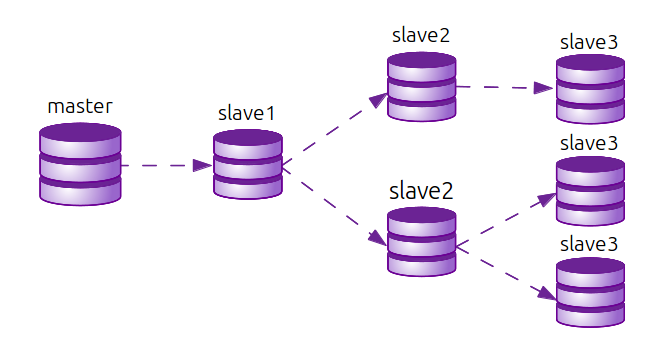
\includegraphics[scale=1]{../../../grafy/obr/schema_kaskadova.png}
            \caption{Ukázka kaskádové replikace}
            \label{kaskadova}
          \end{figure}

Každý databázový server (myšleno SŘDB) si volí terminologii a konkrétní nastavení mírně odlišně. Tato kapitola se snaží popsat chápání replikace co v největší míře obecně s ohledem na použití tohoto pojmu v PostgreSQL. Zcela jinou terminologii, ikdyž založenou na stejných principech, zavádí MS SQL Server, který používá pojmy transakční replikace pro Master-Slave replikace a slučovací replikaci pro Master-Master replikaci. 


